
\textbf{t-SNE comparison (multi-seed).} Figures for EquiSSL-perm seeds 1 and 2 (tsne\_equissl\_seed1.png, tsne\_equissl\_seed2.png) and SANE seeds 1 and 2 (tsne\_sane\_seed1.png, tsne\_sane\_seed2.png) show consistent patterns across seeds: EquiSSL-perm ViT latents are distributed; SANE ViT latents are collapsed.

\begin{figure}[htbp]
\centering
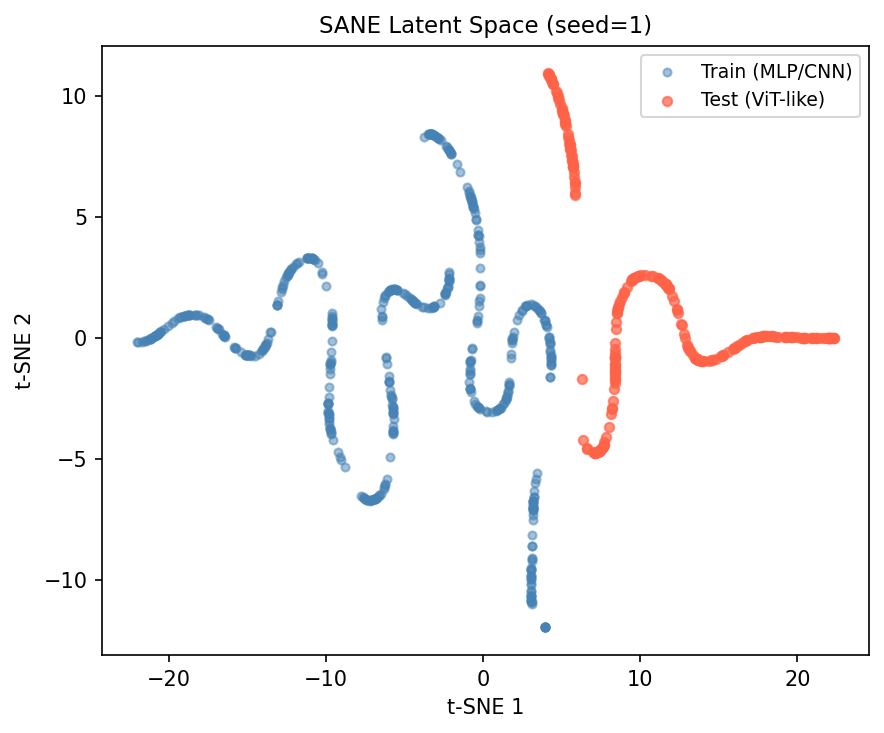
\includegraphics[width=\columnwidth]{figures/tsne_sane_seed1.png}
\caption{SANE t-SNE seed 1}
\label{fig:tsne_sane_seed1}
\end{figure}

\begin{figure}[htbp]
\centering
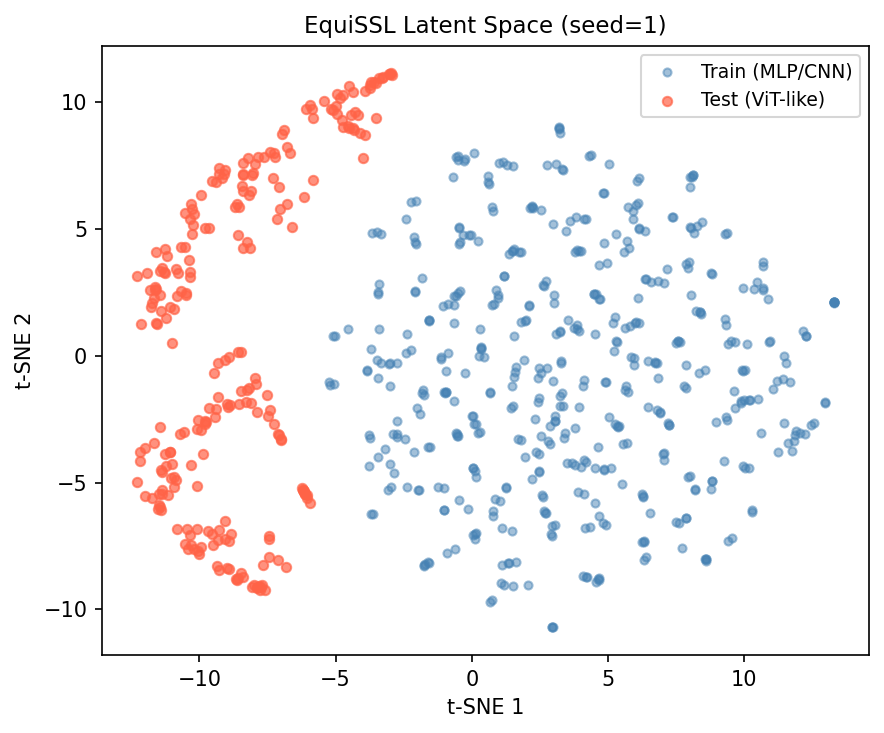
\includegraphics[width=\columnwidth]{figures/tsne_equissl_seed1.png}
\caption{EquiSSL-perm t-SNE seed 1}
\label{fig:tsne_equissl_seed1}
\end{figure}

\textbf{4-panel t-SNE (h-m2).} Figure tsne\_2x2\_panel.png shows EquiSSL and EquiSSL-perm latent spaces side by side on both CNN training zoo and ViT test zoo, enabling direct visual comparison.

\begin{figure}[htbp]
\centering
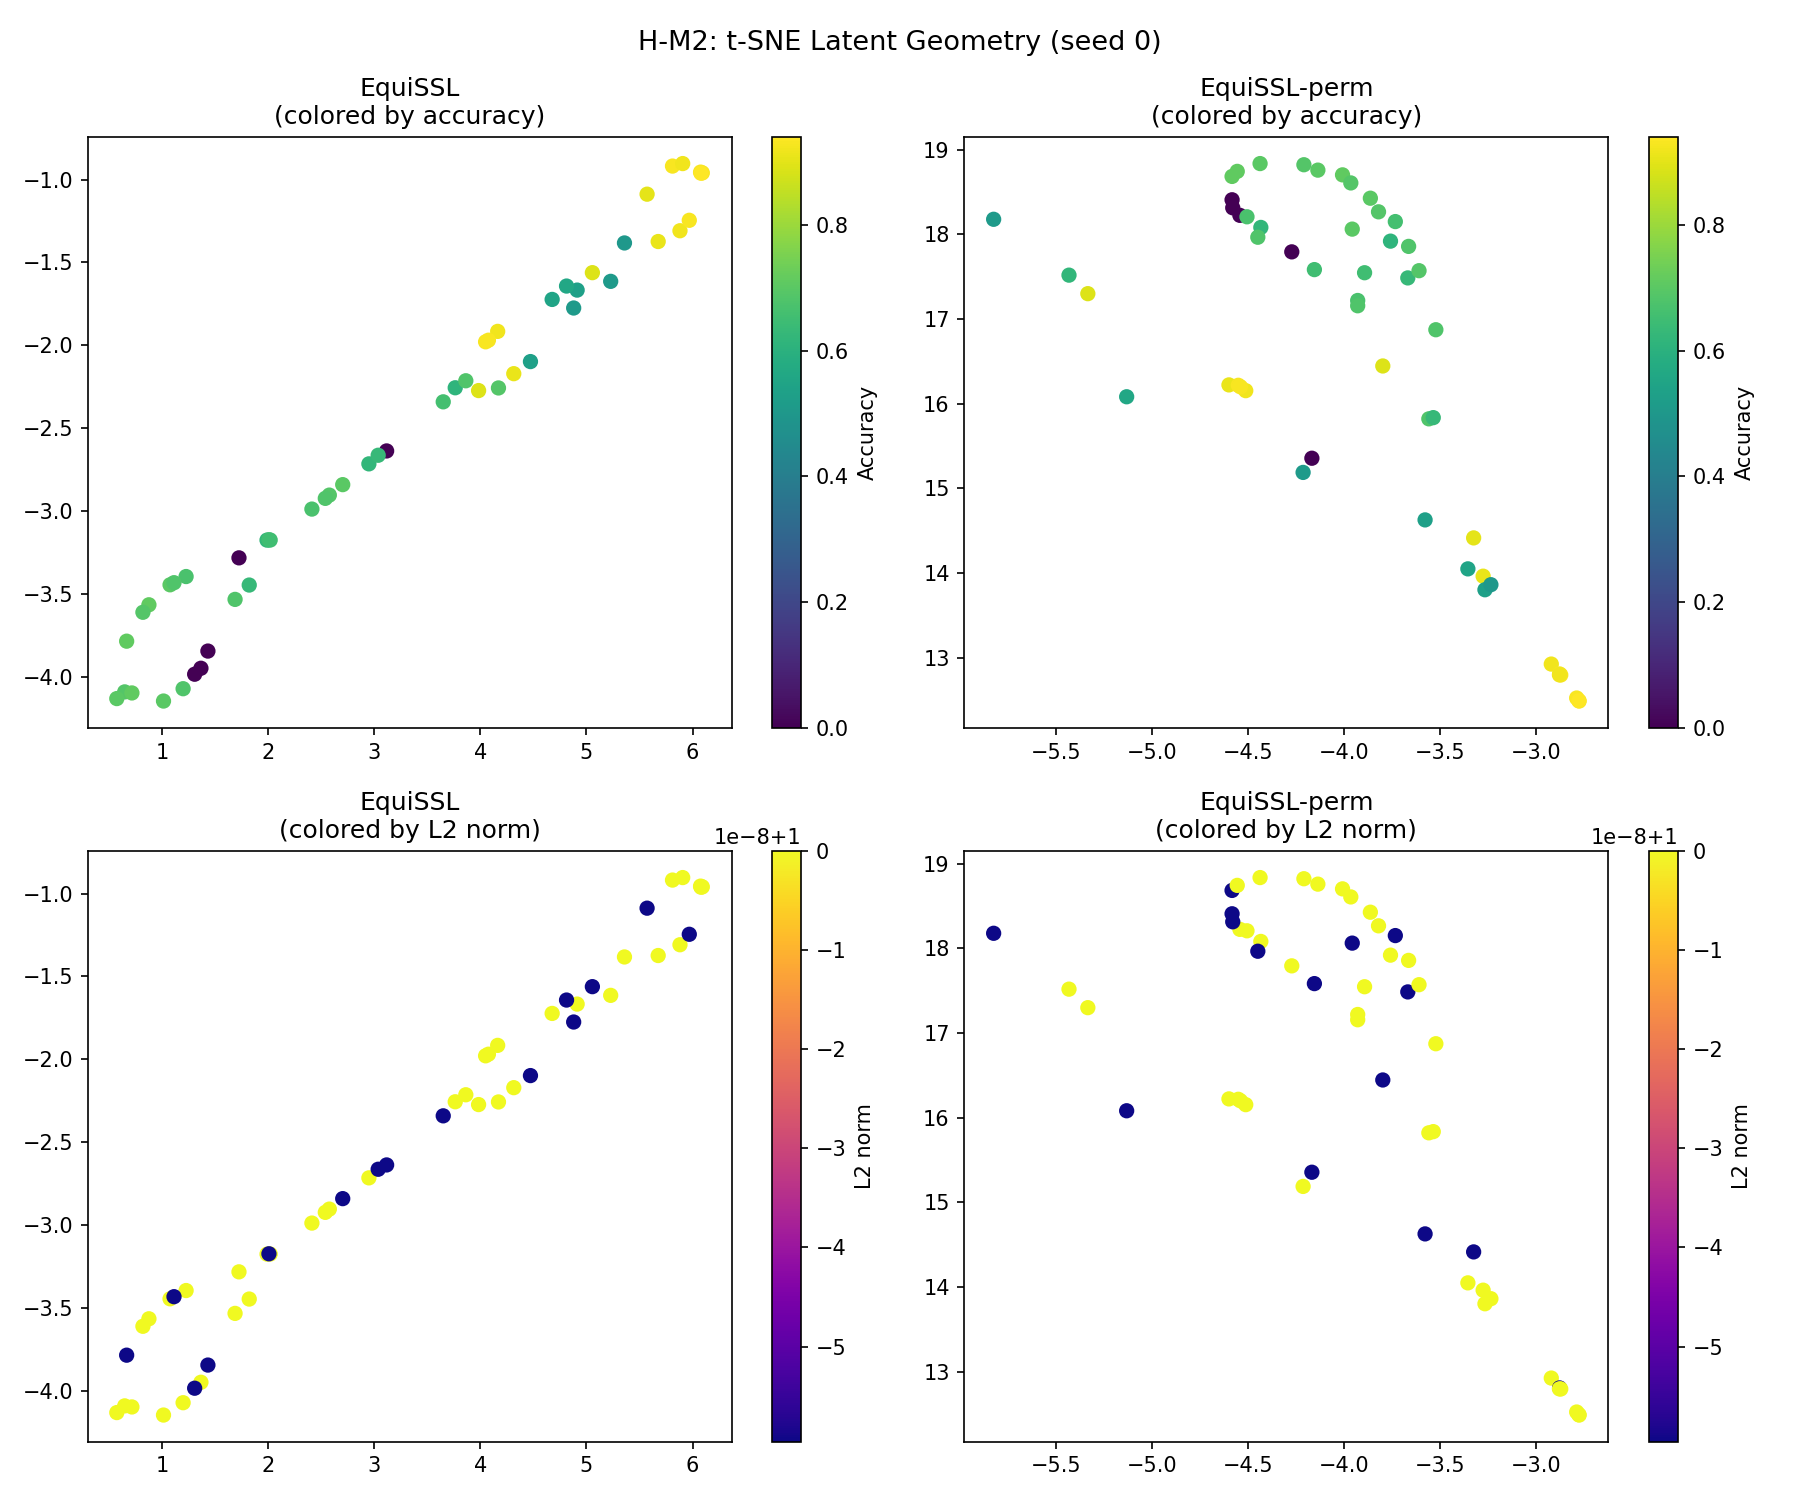
\includegraphics[width=\columnwidth]{figures/tsne_2x2_panel.png}
\caption{4-panel t-SNE: EquiSSL vs EquiSSL-perm (h-m2)}
\label{fig:tsne_2x2_panel}
\end{figure}

\textbf{Interpolation failure detail.} Figure pair\_scatter.png (h-m3) shows the per-pair relationship between acc\_latent and acc\_ws. Figure gate\_comparison.png (h-m3) shows the aggregate comparison.

\begin{figure}[htbp]
\centering
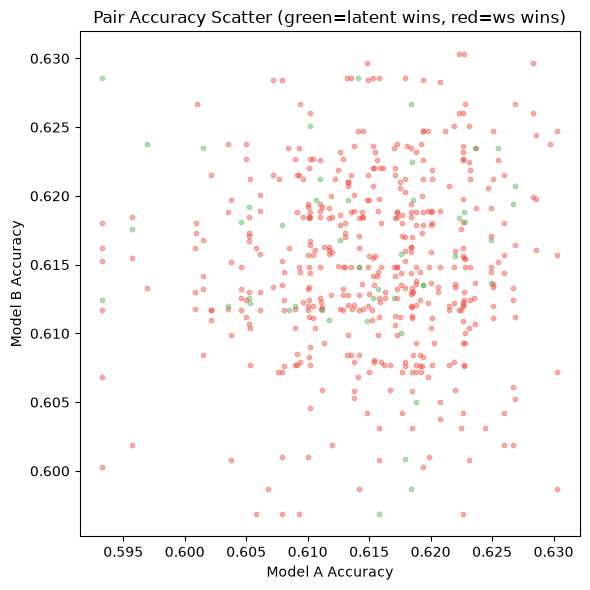
\includegraphics[width=\columnwidth]{figures/pair_scatter.png}
\caption{Interpolation pair scatter (h-m3)}
\label{fig:pair_scatter}
\end{figure}

\textbf{MMD supplementary.} Figure mmd\_comparison.png (h-e1) shows SANE vs. EquiSSL MMD side by side. This figure covers only the two methods for which cross-architecture MMD was computed in h-e1; EquiSSL-perm is not included.

\textbf{Note on MMD incompatibility.} The within-ViT-zoo subpopulation MMD values reported in h-m2 (EquiSSL-perm: 0.203, EquiSSL: 0.431) measure a different quantity --- separation between high- and low-accuracy ViT subgroups within the test zoo --- and are not directly comparable to the cross-architecture MMD values in Table 3. Both are labeled ''MMD'' in the experiment logs; readers should not compare them across experiments.
